\documentclass[a4paper, 11pt]{article}
\usepackage{amsmath, amssymb, amsthm}
\usepackage{xeCJK}
\usepackage{fontspec}
\usepackage{xunicode}
\usepackage{xltxtra}
\usepackage{graphicx}

\setCJKfamilyfont{tt}{SimSun}
\setmainfont{SimSun} 		%默认字体,默认英文字体。
\setCJKmainfont{SimSun} 		%中文默认字体
\setCJKmonofont{SimSun}
\CJKsetecglue{} 			%中英间隔

%\XeTeXlinebreaklocale "zh"  % 表示用中文的断行
%\XeTeXlinebreakskip = 0pt plus 1pt % 多一点调整的空间设置字体。

\newcommand{\cn}{\fontspec{Courier New}}
%字体大小
\newcommand{\ltwo}{\fontsize{18pt}{27pt}\selectfont} 		%小二
\newcommand{\three}{\fontsize{16pt}{24pt}\selectfont}		%三号
\newcommand{\lthree}{\fontsize{15pt}{22.5pt}\selectfont}	%小三
\newcommand{\four}{\fontsize{14pt}{21pt}\selectfont}		%四号
\newcommand{\lfour}{\fontsize{13pt}{18pt}\selectfont}		%小四
\newcommand{\five}{\fontsize{10.5pt}{15.75pt}\selectfont}	%五号
\newcommand{\lfive}{\fontsize{9pt}{13.5pt}\selectfont}		%小五

\usepackage{listings}
\lstset{language=Java}%这条命令可以让LaTeX排版时将C++键字突出显示
\lstset{breaklines}%这条命令可以让LaTeX自动将长的代码行换行排版
%\lstset{extendedchars=false}%这一条命令可以解决代码跨页时,章节标题,页眉等汉字不显示的问题
\lstset{xleftmargin=28pt}
\lstset{tabsize=4}
\lstset{escapechar=`} %中文注释问题
\lstset{columns=flexible}
\lstset{basicstyle=\cn\lfive}

%图,表标题的间距。
\usepackage{caption}
\setlength{\abovecaptionskip}{10pt}
\setlength{\belowcaptionskip}{0pt}
\usepackage{tabularx}

\renewcommand {\tablename}{\five 表}
\renewcommand {\thetable}{\arabic{table}}
\usepackage{booktabs}
\renewcommand {\heavyrulewidth}{1.5pt}	%表格外线宽
\renewcommand {\lightrulewidth}{1pt}	%表格内线宽

\captionsetup{labelsep=space}

%%%%%%%%%%%%%%%%%%%%%%%%
%%%%%%%%%%%正文%%%%%%%%%%
%%%%%%%%%%%%%%%%%%%%%%%%
\begin{document}

\title{{\Huge 算法分析与设计第四次作业\\}}
\author{黄丛宇 2010212439}
\date{\today}

\maketitle

\section{实验环境}
\begin{itemize}
	\item CPU: Intel(R) Core(TM)2 Duo CPU T5870 2.00GHz
	\item MEM: 1GB
	\item OS : Debian 5.0 (1GB swap)
	\item Java: java version "1.6.0\_21"
\end{itemize}
\section{Exercise 15.4-4}

由算法可知,在算法执行过程中,算法每次循环只使用当前行和前一行的数据。因此,可以使用一个只有两行的
二维滚动数组来存储数据。另外,使用一个变量,标记那一行是当前行,则另一行是前一行。由于算法中两个循环
谁在外边谁在里面不应想算法的正确性,因此可以min(m,n)放在内循环中。这样,滚动数据只需要2*min(n,m)
的长度,外加一个$O(1)$的标记变量。

可以进一步将两行的二维数组变成一个一维的数组。观察算法可得,内循环的每次运算中,假如当前要计算的元素
是c[i,j],那么计算只使用了c[i-1, j-1],c[i-1, j]和c[i, j-1]。当使用一维数组的时候,假设当前
计算的元素是c'[i],那么c'[i - 1]存放的就是原来的c[i-1, j],而当前的c'[i]中存放的是c[i, j-1]
的值,现在只缺少c[i-1, j-1],这个值恰好就是c[i-1]中存放的前一个值。因此,可以使用一个变量,在
计算c[i-1]的时候,将c[i-1]的前一个值保存起来,给c[i]使用。同样,计算c[i]的时候,在覆盖c[i]之前
,将其值保存在这个变量中。同理,数组的长度为min(n,m),因此,算法只需要min(n,m)长度的数组外加一个
$O(1)$的标记变量。

\section{Exercise 15.4-6}

定义b[k]表示以s[k]结尾的最长递增子序列的长度,则状态转移方程如下:
\begin{displaymath}
                     b[k]=max(max(b[j]|s[j]<s[k],j<k)+1,1);
\end{displaymath}  	

在a[k]前面找到满足a[j]<a[k]的最大b[j],然后把a[k]接在它的后面,可得到以a[k]结尾的最长递增子序
列的长度,或者a[k]前面没有比它小的a[j],那么这时a[k]自成一序列,长度为1。最后整个数列的最长递增
子序列即为max(b[k]|0<=k<=n-1);

在寻找最大的b[j]的时候,如果使用顺序查找,则算法复杂度为$O(n ^ 2)$,因此使用二分查找降低时间复杂
度。

引入一个新的数组c。c中元素满足$c[b[k]]=a[k]$,即当递增子序列的长度为b[k]时子序列的末尾元素为
$c[b[k]]=a[k]$。算法中对c的修改可以保证c是有序的。如果有多个相同长度的递增子列,那么对应的位置
存放的是最后出现的那个子列的最后一个元素。c[1]=s[0],c[0]=0。c[0]作为二分查找的哨兵使用。

核心代码如下:
\begin{lstlisting}
	public static int getLISLen(final int[] s, int[] lis)
	{
		if (null == s) {
			return -1;
		}
		c = new int[s.length + 1];
		cindex = new int[s.length + 1];
		pre = new int[s.length];
		
		//`初始化`
       		cindex[0] = -1;
       		for(int i = 0; i < s.length; ++i){
       			pre[i] = -1;
       			cindex[i + 1] = -1;
       		}
       		
       		c[0] = 0; //`这个元素作为一个哨兵。在二分查找中使用。`
       		c[1] = s[0];
       		cindex[1] = 0;
       		len = 1;	//`此时只有`c[1]`求出来,最长递增子序列的长度为1.`
		int j;
		for(int i = 1; i < s.length; ++i){
			j = binarySearch(c, len, s[i]);
			c[j] = s[i];
			cindex[j] = i;
			/*
			 * `以`s[i]`结尾的最长子串的倒数第二个元素是`c[j-1]`。`
			 */
			pre[i] = cindex[j - 1];
			if(len < j){
				len = j;
				lastIndex = i;
			}
			
		}
		getSubsquence(s, lis);
		return len;
	}
	/**
	 * `二分查找。返回值表示`n`在数组`a`中的位置。如果在数组中有元素等于`n
	 * `那么返回最后一个等于`n`的元素的下一个位置。`
	 * @param a  `数组`a
	 * @param len `数组`a`中数据的个数`
	 * @param n  `需要查找的元素`
	 * @return
	 */
	private static int binarySearch(final int[] a, int len, int n)
	{
		if (n < 0) {
			return -1;
		}

		int left = 0, right = len;
		int mid = (left + right) / 2;

		while (left <= right) {
			/*
			 * `等于是为了处理"两个相等的元素"也是递增序列的情况`
			 */
			if (n >= a[mid]){
				left = mid + 1;
			}
			else if (n < a[mid]){
				right = mid - 1;
			}
			
			mid = (left + right) / 2;
		}
		return left;
	}
	
	/**
	 * `构造其中一个最长递增子列。`
	 * @param s `原始序列。`
	 * @param lis `最长子列`
	 */
	private static void getSubsquence(final int[] s, int[] lis)
	{
		int pr;
		int index = len;
		pr = lastIndex;
		do{
			lis[--index] = s[pr];
			pr = pre[pr];
		}while(pr != -1);		
	}
	
	//`最长递增子列的长度`
	private static int len = 0;
	//`最长递增子列最后一个元素的位置。`
	private static int lastIndex = -1;
	/*
	 * c[i]=a[j],`表示`c[i]`中存储的是长度为`i`的最长递增子列的最后一个元素。`
	 * `并且,`c`中存放的就是最长递增子列。`
	 * c`从`1`开始,`c[0]`最为哨兵在二分搜索中使用`
	 */
	private static int[] c;
	/*
	 * cindex[i]`存储`c[i]`对应的元素在序列中的位置。`
	 */
	private static int[] cindex;
	/*
	 * pre[i]`表示`s[i]`所在的最长递增子列的前一个元素的位置。`
	 * `注,这个最长子列可能不是`s`的最长子列,只是包含`s[i]`中所有`
	 * `递增子列最长的。`
	 */
	private static int[] pre;
\end{lstlisting}

使用一个pre数组保存每个元素所在的最长递增子列的前一个元素的位置。pre[i]表示s[i]所在的最长递增
子列中,s[i]前一个元素的下标。使用pre数组,可以在$O(n)$的时间内构造出一个最长的递增子列。

运行结果如下:

\begin{figure}[htbp]
\centering
\caption{运行结果}
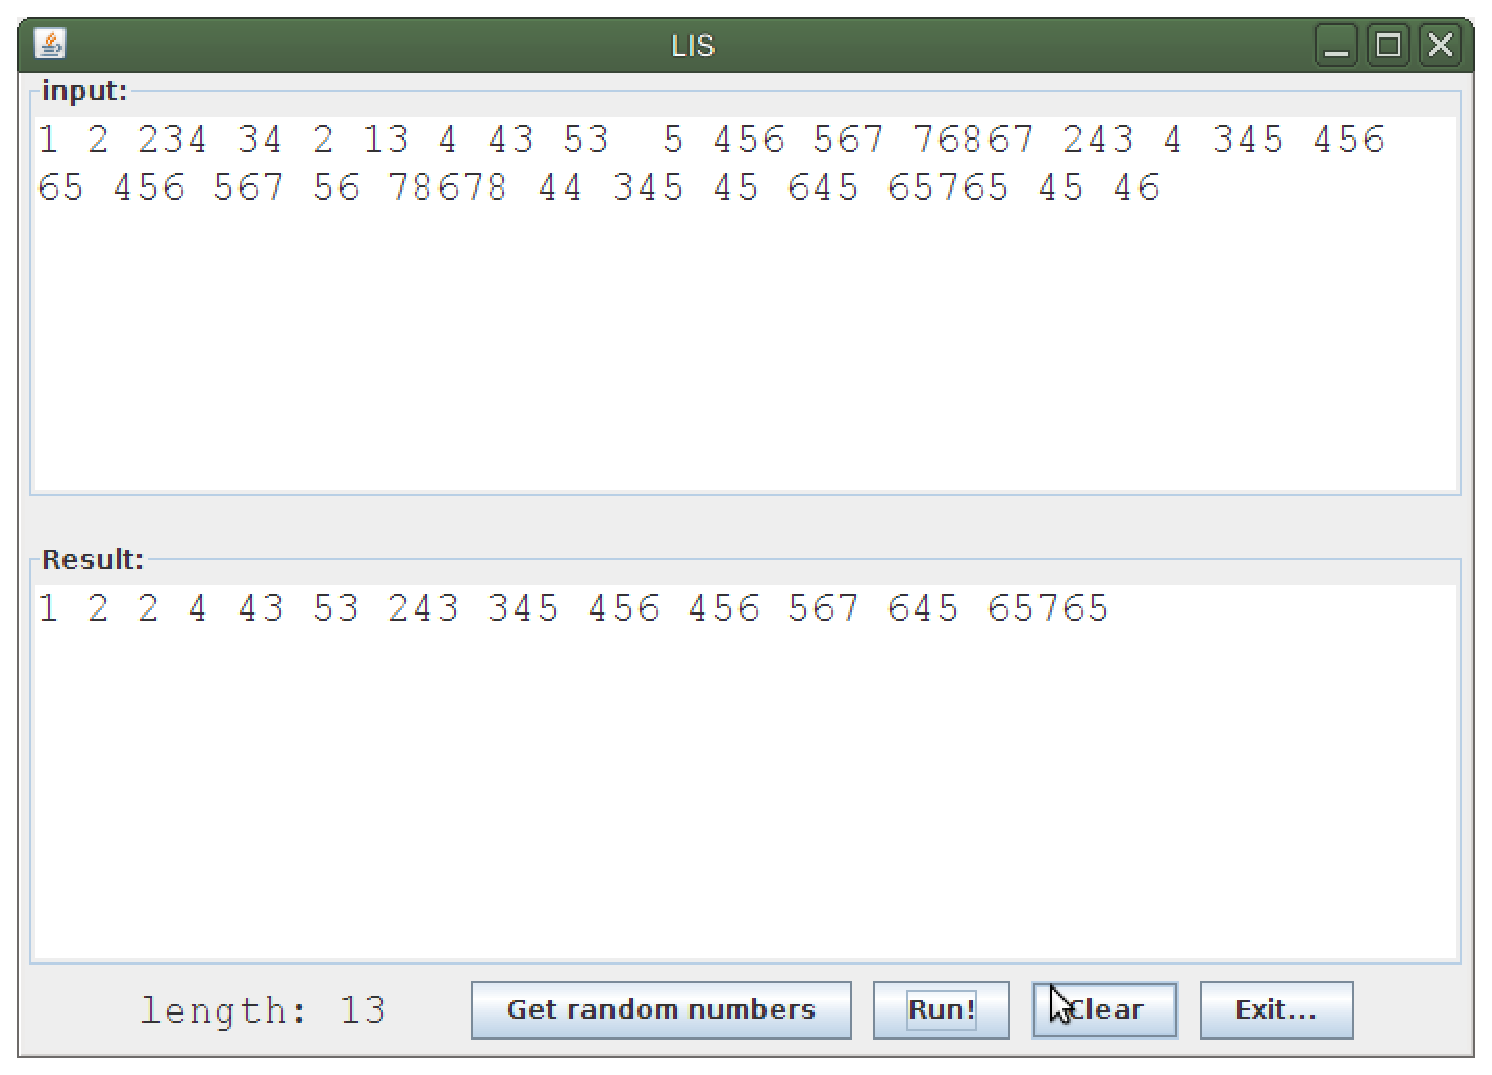
\includegraphics[height=8cm, width=11cm]{LIS.eps}
\end{figure}

\section{Problem 15-1 bitonic tours}

对所有点按x坐标排序。$T(i)$表示前i个点的最短路径,那么$T(i)$可以从$T(i - 1)$构造出。从
$T(i-1)$中选出一条边,使得从$T(i-1)$删除这条边并加上这条边的两个端点到点i的两条边之后,
路径距离最短。从$T(i-1)$删除这条边并加上两条新边后就得到了$T(i)$。

算法如下:
\begin{verbatim}
    对所有的点按x坐标排序,将排好序的点存入数组p。
    path存储当前最短路径。
    path_len为当前最短路径的长度
	
    边(p[0],p[1])存入path中。
    path_len等于边(p[0],p[1])的长度
	
    for(i从1到n-1)
        for(path中的每一条边(p[x], p[y]))
            计算从path删除边(p[x], p[y]),并加上边(p[x], p[i])和
            边(p[i], p[y])后的路径长度。
            记录这个路径的最小值和要删除的边。
        从path中删除这个边,并加上新的两条边。
        更新path_len的值。
\end{verbatim}
	
最终,path中存储最短路径的所有边,path\_len存储最短路径长度。

path可以使用一个双向连表,插入和删除的时间可以在$O(1)$内实现。排序算法使用快速排序,时间
$O(nlgn)$。外循环需要n-1次,内循环要i - 2次,因此,算法的时间复杂度是$O(n ^ 2)$

\section{Problem 15-6 checker}

用一个n×n的二维数组c表示checkerboader。那么,对于格子c[i][j],checker只可能从c[i][j-1],
c[i-1][j-1]和c[i+1][j-1]三个格子移动过来。用一个二维数组b表示到达每个格子所能获得的最大钱数。
b[i][j]表示checker到达c[i][j]时所能获得的最大钱数。每一个格子的标号用i*n+j表示。可以得到如下
的递推方程:
\begin{align*}
                     b[i][j]=max(b[i-1][j]+p((i-1)*n+j, i*n+j)\\
                     		,b[i-1][j-1]+p((i-1)*n+j-1, i*n+j)\\
                     		,b[i-1][j+1]+p((i+1)*n+j+1, i*n+j))
\end{align*}

算法如下:
\begin{verbatim}
    maxValue = -1
    b存储checker到达每个格子所得到的最大值。
    for(i=1; i < n; ++i)
        for(j=0; j < n; ++j)
            b[i][j] = max(b[i-1][j]+p((i-1)*n+j, i*n+j)
                        ,b[i-1][j-1]+p((i-1)*n+j-1, i*n+j)
                        ,b[i-1][j+1]+p((i+1)*n+j+1, i*n+j));

    for(i=0; i < n; ++i)
        if(maxValue < b[n-1][i])
        maxValue = b[n-1][i]
\end{verbatim}
	
外层循环和内层循环分别是n-1次和n次,因此算法的复杂度是$O(n^2)$
\end{document}
